\documentclass[]{article}
\usepackage{lmodern}
\usepackage{amssymb,amsmath}
\usepackage{ifxetex,ifluatex}
\usepackage{fixltx2e} % provides \textsubscript
\ifnum 0\ifxetex 1\fi\ifluatex 1\fi=0 % if pdftex
  \usepackage[T1]{fontenc}
  \usepackage[utf8]{inputenc}
\else % if luatex or xelatex
  \ifxetex
    \usepackage{mathspec}
  \else
    \usepackage{fontspec}
  \fi
  \defaultfontfeatures{Ligatures=TeX,Scale=MatchLowercase}
\fi
% use upquote if available, for straight quotes in verbatim environments
\IfFileExists{upquote.sty}{\usepackage{upquote}}{}
% use microtype if available
\IfFileExists{microtype.sty}{%
\usepackage{microtype}
\UseMicrotypeSet[protrusion]{basicmath} % disable protrusion for tt fonts
}{}
\usepackage[margin=1in]{geometry}
\usepackage{hyperref}
\hypersetup{unicode=true,
            pdftitle={DATA 609 - Homework 5},
            pdfauthor={Joshua Sturm},
            pdfborder={0 0 0},
            breaklinks=true}
\urlstyle{same}  % don't use monospace font for urls
\usepackage{graphicx,grffile}
\makeatletter
\def\maxwidth{\ifdim\Gin@nat@width>\linewidth\linewidth\else\Gin@nat@width\fi}
\def\maxheight{\ifdim\Gin@nat@height>\textheight\textheight\else\Gin@nat@height\fi}
\makeatother
% Scale images if necessary, so that they will not overflow the page
% margins by default, and it is still possible to overwrite the defaults
% using explicit options in \includegraphics[width, height, ...]{}
\setkeys{Gin}{width=\maxwidth,height=\maxheight,keepaspectratio}
\IfFileExists{parskip.sty}{%
\usepackage{parskip}
}{% else
\setlength{\parindent}{0pt}
\setlength{\parskip}{6pt plus 2pt minus 1pt}
}
\setlength{\emergencystretch}{3em}  % prevent overfull lines
\providecommand{\tightlist}{%
  \setlength{\itemsep}{0pt}\setlength{\parskip}{0pt}}
\setcounter{secnumdepth}{0}
% Redefines (sub)paragraphs to behave more like sections
\ifx\paragraph\undefined\else
\let\oldparagraph\paragraph
\renewcommand{\paragraph}[1]{\oldparagraph{#1}\mbox{}}
\fi
\ifx\subparagraph\undefined\else
\let\oldsubparagraph\subparagraph
\renewcommand{\subparagraph}[1]{\oldsubparagraph{#1}\mbox{}}
\fi

%%% Use protect on footnotes to avoid problems with footnotes in titles
\let\rmarkdownfootnote\footnote%
\def\footnote{\protect\rmarkdownfootnote}

%%% Change title format to be more compact
\usepackage{titling}

% Create subtitle command for use in maketitle
\newcommand{\subtitle}[1]{
  \posttitle{
    \begin{center}\large#1\end{center}
    }
}

\setlength{\droptitle}{-2em}

  \title{DATA 609 - Homework 5}
    \pretitle{\vspace{\droptitle}\centering\huge}
  \posttitle{\par}
    \author{Joshua Sturm}
    \preauthor{\centering\large\emph}
  \postauthor{\par}
      \predate{\centering\large\emph}
  \postdate{\par}
    \date{October 15, 2018}


\begin{document}
\maketitle

\hypertarget{chapter-6-problems}{%
\section{Chapter 6 problems}\label{chapter-6-problems}}

\hypertarget{page-228-exercise-1}{%
\subsection{1 (Page 228, exercise \#1)}\label{page-228-exercise-1}}

Consider a model for the long-term dining behavior of the students at
College USA. It is found that 25\% of the students who eat at the
college's Grease Dining Hall return to eat there again, whereas those
who eat at Sweet Dining Hall have a 93\% return rate. These are the only
two dining halls available on campus, and assume that all students eat
at one of these halls. Formulate a model to solve for the long-term
percentage of students eating at each hall.

\hypertarget{solution}{%
\subsubsection{1 Solution}\label{solution}}

The transitional matrix is

\begin{verbatim}
## Markov Chain 1 
##  A  2 - dimensional discrete Markov Chain defined by the following states: 
##  Grease, Sweet 
##  The transition matrix  (by rows)  is defined as follows: 
##        Grease Sweet
## Grease   0.25  0.75
## Sweet    0.07  0.93
\end{verbatim}

And the markov chain is show plotted below:

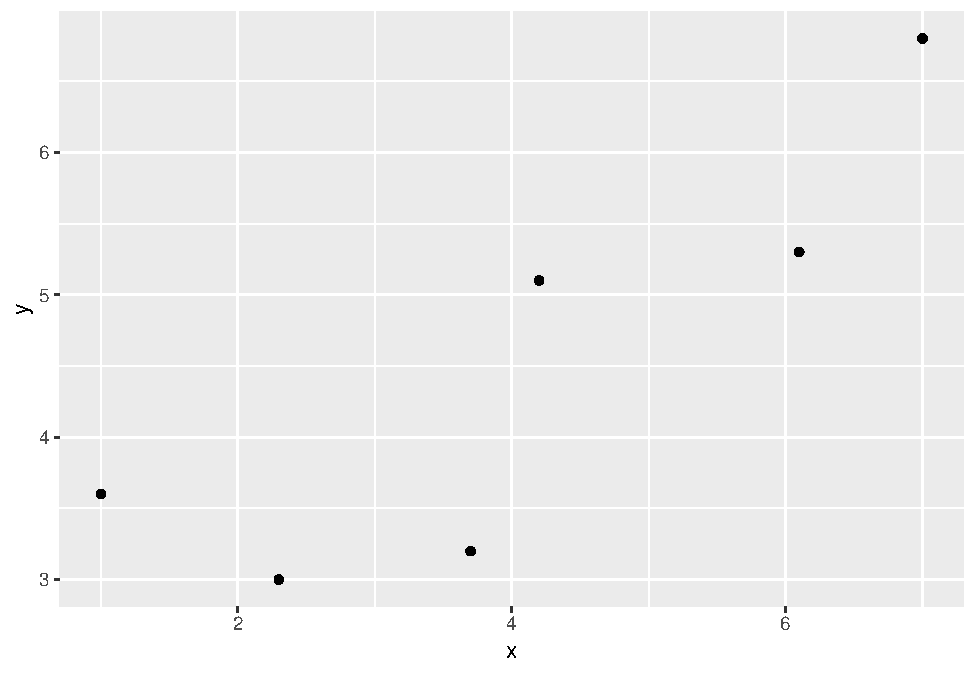
\includegraphics{Joshua_Sturm_Homework5_files/figure-latex/unnamed-chunk-2-1.pdf}

Let \(G_n\) = the percentage of students who eat at Grease Dining Hall
at the end of period \(n\). \textbackslash{} Let \(S_n\) = the
percentage of students who eat at Sweet DininG Hall at the end of period
\(n\).

Then,

\(G_{n+1} = 0.25G_n + 0.07S_n\) \textbackslash{}
\(S_{n+1} = 0.75G_n + 0.93S_n\)

We can visualize the model's prediction over time.

\begin{verbatim}
##     n    Grease     Sweet
## 1   0 0.5000000 0.5000000
## 2   1 0.1600000 0.8400000
## 3   2 0.0988000 0.9012000
## 4   3 0.0877840 0.9122160
## 5   4 0.0858011 0.9141989
## 6   5 0.0854442 0.9145558
## 7   6 0.0853800 0.9146200
## 8   7 0.0853684 0.9146316
## 9   8 0.0853663 0.9146337
## 10  9 0.0853659 0.9146341
## 11 10 0.0853659 0.9146341
\end{verbatim}

We can see the model converges after 10 timesteps.

To view this graphically:

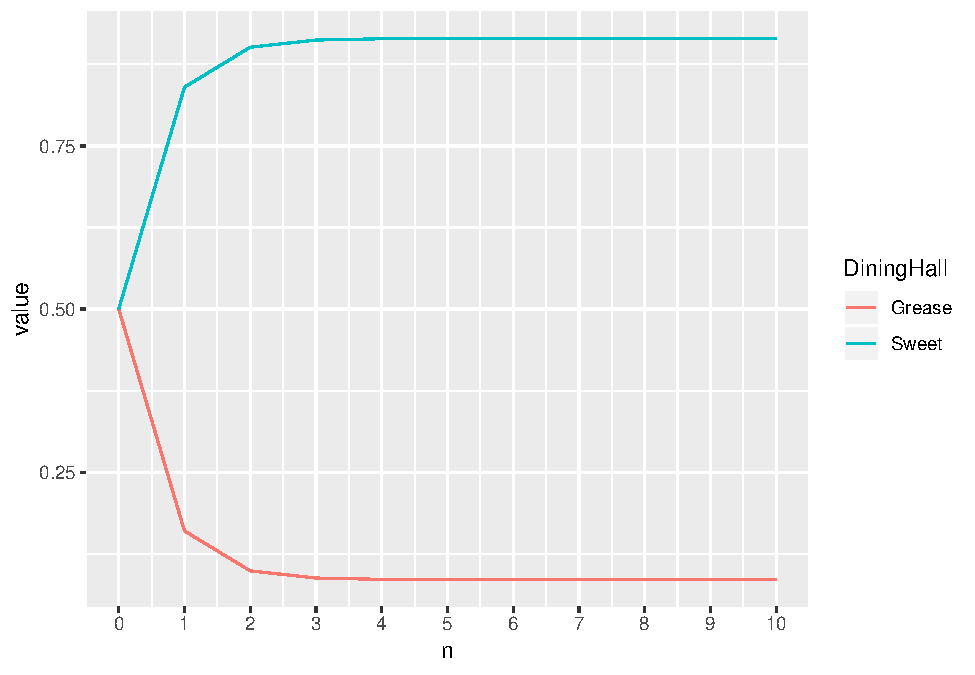
\includegraphics{Joshua_Sturm_Homework5_files/figure-latex/unnamed-chunk-4-1.pdf}

\hypertarget{page-232-exercise-1}{%
\subsection{2 (Page 232, exercise \#1)}\label{page-232-exercise-1}}

Consider a stereo with CD player, FM-AM radio tuner, speakers (dual),
and power amplifier (PA) components, as displayed with the reliabilities
shown in Figure 6.11. Determine the system's reliability. What
assumptions are required in your model?

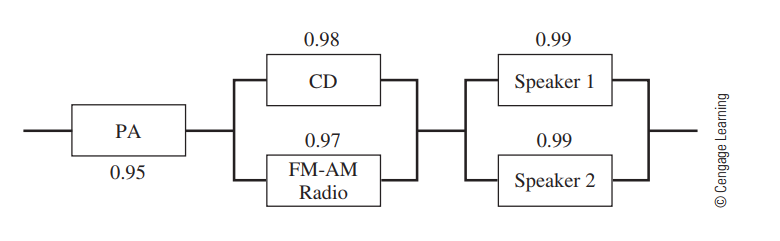
\includegraphics{image2.png}

\hypertarget{solution-1}{%
\subsubsection{2 Solution}\label{solution-1}}

We can divide it into three parts: - The PA system - The CD and FM-AM
radio - Speaker 1 and speaker 2

Let \(R_1, R_2,\) and \(R_3\) represent the above three parts,
respectively.

Then,

\begin{align*}
R_1 &= 0.95 \\
R_2 &= R_2(1) + R_2(2) - (R_2(1)\times R_2(2)) = 0.98 + 0.97 - (0.98\times 0.97) = 0.9994 \\
R_3 &= R_3(1) + R_3(2) - (R_3(1)\times R_3(2)) = 0.99 + 0.99 - (0.99\times 0.99) = 0.9999
\end{align*}

The reliability of the system as whole is \(R_1 \times R_2 \times R_3\).

\(R = 0.95 \times 0.9994 \times 0.9999 =\) 0.9493351.

References: - \url{https://rpubs.com/JanpuHou/326048} -
\url{https://www.datacamp.com/community/tutorials/markov-chain-analysis-r}


\end{document}
